\documentclass[12 pt]{article}
\usepackage{amssymb,amsmath,amstext,amsgen,amsbsy,amsopn,amsfonts,graphicx,theorem, anysize,multicol,algorithm, algorithmic, CJKutf8}
%\marginsize{0.5in}{0.5in}{0.5in}{0.5in}
%\marginsize{left}{right}{top}{bottom}
%\usepackage[lmargin=2cm,,rmargin=2cm,tmargin=2cm,bmargin=2cm]{geometry}
\usepackage[margin=1in]{geometry}

\begin{document}
\bibliographystyle{acm}
\title{UROP I Progress Report \\ Word Sense Disambiguation}
\author{Heng Low Wee \\ U096901R}
\date{}
\maketitle
%\begin{abstract}
%Lorem ipsum dolor sit amet, consectetur adipisicing elit, sed do eiusmod tempor incididunt ut labore et dolore magna aliqua. Ut enim ad minim veniam, quis nostrud exercitation ullamco laboris nisi ut aliquip ex ea commodo consequat. Duis aute irure dolor in reprehenderit in voluptate velit esse cillum dolore eu fugiat nulla pariatur. Excepteur sint occaecat cupidatat non proident, sunt in culpa qui officia deserunt mollit anim id est laborum.
%\end{abstract}

\section{Introduction}
\label{introduction}
\paragraph{}
In any human language, there are some words, or even phrases, that have multiple interpretations depending on the context in which a word is used. These words are called homographs, and have multiple meanings (or \textit{senses}), making language itself ambiguous. Here are some examples:
\begin{enumerate}
\item{She is interested in the \textit{interest} rates of the bank.}
\item{He developed an \textit{interest} in art.}
\end{enumerate}
\paragraph{}
Observe that the word \textit{interest} in the two sentences clearly have different meanings. This is the ambiguity we are talking about. Paraphrasing Weaver \cite{weaver}, if we examine some text only \textit{one} word at a time, it is impossible to determine the meaning of it. Only by looking at its surrounding words then can one decide its meaning. It is almost an unconscious act for a human to interpret the word's correct sense. But because human languages are complex, a machine need to run through a series of analytical processes before it can guess the best answer. In general, this process is \textit{Word Sense Disambiguation} (\textit{WSD}). More formally, WSD is the process of deciphering the intended meaning of a homographic word(s) in a given context.
There are four conventional methods to WSD, namely:
\begin{enumerate}
\item{Dictionary-based \& knowledge-based \\ This method relies mainly on dictionaries and lexical knowledge bases to disambiguate senses. The Lesk Algorithm \cite{michaellesk} is such a method. Satanjeev \& Ted adapted the Lesk Algorithm but instead of using a standard dictionary, they used WordNet \cite{wordnet} as a source of words' senses (for details, refer to \cite{lesk}). After evaluation testings, it was found that their implementation outperformed a more traditional Lesk approach with an accuracy rate of 32\%, double of the traditional approach. This demonstrated the fact that an approach that integrates WordNet, or other lexical databases, would be able to achieve a higher rate of accuracy in WSD.}
\item{Supervised \\ Generally, this method relies on manually sense-tagged corpora. Using manually sense-tagged corpora allows supervised methods to achieve a higher accuracy as compared to most unsupervised methods. The downside of using manually sense-tagged corpora, however, is its high costs and labour intensiveness to create.}
\item{Semi-supervised \\
This method makes use of both labeled and unlabeled data. Similarly, it refers to using multiple untagged corpora to provide concurrent information to supplement a tagged corpus.}
\item{Unsupervised \\ This is probably the most challenging among all the approaches to WSD. This method may also be closely related to \textit{Word Sense Induction}, where senses can be induced from analyzing the words in a given text. Schutze \cite{hinrich} described a disambiguation algorithm based on clustering words, and then senses are interpreted as a cluster of similar context of an ambiguous word. To determine the senses, some algorithms may also map the words to a collection of senses. Mihalcea \cite{wikipedia} described an unsupervised approach by using the articles on Wikipedia, together with mapping of senses with a WordNet resource. It addressed the issue of \textit{knowledge acquisition bottleneck}, as Wikipedia serves as a dynamic source for senses because it is updated by users all around the world regularly. More importantly, it addresses the case where languages are gaining new words, and that words are gaining new senses, a common thing in today's modern society.}
\end{enumerate}
%We want to study how to make bilingual translations better, not just word-for-word translations but to retain the correct senses and context as well. Hence, the topic we will be focusing on is \textit{Cross Lingual Word Sense Disambiguation}, in particular between English and Chinese languages.
\paragraph{}
There are many applications that are related to WSD. For instance, if search engines are able to identify the correct sense in the search words, search results will be more accurate and relevant. Another application would be language translations. During the translation process from English to Chinese and vice versa, words that are ambiguous would usually end up with an entirely wrong translation output. For instance, the translation for \textit{interest}, as mentioned in the first example, might be \begin{CJK}{UTF8}{gbsn}兴趣\end{CJK}, which is more related to the term ``hobby''. Also, we wish for the system to be able to handle new words and new senses in human languages. In this paper, we introduce an existing translation tool, DiCE Translator, that allows users to translate text on a webpage from English to Chinese and vice versa. We also explore some methods to integrate WSD so as to improve the accuracy of bilingual translations by retaining the original context.

\section{Related Work}
\subsection{Word Sense Tagging using Parallel Corpora}
\label{parallel}
\paragraph{}
Supervised word sense disambiguation systems rely heavily on manually sense-tagged corpora, and to produce more reliable results they need high quality annotations. However, manual tagging is very labour intensive and costly. It is also very impractical as doubling the training corpora only reduces errors by 3 to 4\% \cite{yarowsky}.
\paragraph{}
Diab \& Resnik described a form of automated annotation and sense-tagging by analyzing an ambiguous word's translations in a second language \cite{parallel}.
Their approach involves two languages, for example English and French. The first step is to identify the target words and their corresponding translations in the source corpus. Word alignment is carried out and the corresponding positions of a target word in both languages are captured. Then, grouping the target words into \textit{target sets}.  Next, in each set consider all possible senses for each word and then tag a word with the sense most similar to the other words. Last, they make use of the sense tags in the target sets and project them to the source corpus. (for details, refer to \cite{parallel})
%\paragraph{}
%The advantage of this approach is that it attempts to eliminate the need to carry out manual sense-tagging or annotation. Automation would address the issue about this task being labour-intensive and costly. One disadvantage, however, might be the reduction of accuracy in the tagging and annotating. A solution may be to require gold-standard sense-tags, as mentioned in \cite{parallel}.
%\paragraph{}
%We highlighted this work written by Diab \& Resnik \cite{parallel} precisely because their approach involves the usage of parallel corpora, or in other words, two languages. The general idea of their work is about sense-tagging another corpus using one that has already been sense-tagged. Adapting to this, possibly, we can construct a English-Chinese parallel, which will capture the Chinese translations that are derived (with similar sense or context) from an English word and vice versa. This essentially will improve the quality of bilingual translations.

\subsection{Using Wikipedia for Automatic Word Sense Disambiguation}
\label{wikipedia}
\paragraph{}
Wikipedia articles, manually created by users, are generally correct in terms of its contents. Some examples of Wikipedia links (on an article), in the \textit{MediaWiki} syntax, are \textbf{[[bar(law)$|$bar]]} and \textbf{[[bar(counter)$|$bar]]}. The senses of the word \textit{bar}, namely \textit{law} and \textit{counter}, can be derived by extracting them from the annotated links. Mihalcea \cite{wikipedia} made use of this information and described an approach to build a sense-tagged corpora using Wikipedia articles. It begins with extracting all paragraphs from Wikipedia that contain the occurrences of a given word. It follows that the senses of each word are extracted, then mapped onto their corresponding WordNet senses. Then, the approach moves on into the disambiguation algorithm \cite{wikipedia}. A target text is tokenized, and each token is tagged with its part-of-speech information. Then, collocations are identified. Next, local and topical features are extracted from the context of the ambiguous word. This set of features is similar to the one used by Ng \& Lee \cite{exemplar}. (for details, refer to \cite{wikipedia})
%The approach begins with deriving the sense-tagged corpora. As described by Mihalcea, there are 3 main steps \cite{wikipedia}:
%
%\begin{enumerate}
%\item{(Starting with a given ambiguous word) Extract all the paragraphs in Wikipedia that contain an occurrence of the mentioned word}
%\item{Collect all possible senses from the annotated links. E.g. \textit{law} from \textbf{[[bar(law)$|$bar]]}}
%\item{Map each sense to their corresponding WordNet sense}
%\end{enumerate}
%\paragraph{}
%The advantage of this method is it addresses the \textit{knowledge acquisition bottleneck} issue. The dynamic nature of Wikipedia makes it extensible. Therefore, by using Wikipedia as a corpus, one can be sure that it will always be up-to-date and will contain any new words or new senses. A disadvantage, however, is data inconsistency. Different users might use a different name for the same object or entity. For example, \textit{handphone} and \textit{mobile phone}. This also relates back to the fact that there are new words or senses emerging regularly in today's modern language.
%To tackle this, Wikipedia has disambiguation pages for ambiguous words. To put it simply, these pages contain the list of links leading to the various senses of the word. Yet, however, Mihalcea did not make use of these pages in the described approach. Instead, Mihalcea suggested capturing all possible meanings of ambiguous words from their articles, similar to the idea of capturing the raw data ourselves. One of the reasons was that the links found on these disambiguation pages are not directly linked with ambiguous words. So these pages might not contain all the various senses of a particular word.
%\paragraph{}
%We can observe that this approach would have the flexibility to handle new words and senses. This is because, considering how popular Wikipedia is, any new word or sense used by people, say \textit{tweet} (a post on Twitter), would most likely appear on Wikipedia faster than any formal dictionary databases. But of course, we must also consider the fact that if the number of new words and senses grows as fast as the number of articles, there may be a need to re-construct the sense-tagged corpus. Hence, design considerations for the corpus must include \textit{expandability}. Alternatively, we may use the APIs on MediaWiki to send a query request for a given word, and with some parsing of the output we can extract the needed information. Thus, we can build a real-time WSD system that is highly independent of lexical databases and corpora. Performance issues aside, this could minimize the need to reconstruct a Wikipedia-based corpus on an occasional basis.
%Wikipedia currently supports more than a hundred languages. In this review, however, we are interested in English and Chinese. With English having more than $1,000,000$ articles and Chinese having more than $100,000$ articles\footnote{Statistics from http://www.wikipedia.org/}, Wikipedia will definitely serve as a valuable choice of resource. Apart from the WSD approach described in Michalcea's work \cite{wikipedia}, Wikipedia, or Wiktionary to be specific, also provides more detailed information like pronunciation, sample sentences, synonyms and most importantly, translations. The good part about these translations is that they are already sense-related to the word in the original language, which simply makes these translations more relevant and less redundant.

\subsection{Word Sense Disambiguation using Dependency Knowledge}
\label{treematching}
%In \cite{unsupervised}, the authors highlighted an important problem faced by WSD and Artificial Intelligence (AI) systems: how to overcome the \textit{knowledge acquisition bottleneck} (which can be related to \textit{sense-tagged data bottleneck} mentioned in Section \ref{introduction}). In other words, a WSD must maintain a dynamic and updated source from which it retrieves the necessary information needed to disambiguate words.
%\\
%\\
\paragraph{}
Similar to Section \ref{wikipedia}, this approach described by \cite{unsupervised} begins with the construction of the corpus. In short, ambiguous words are sent to Web search engines to retrieve the relevant pages. These pages are cleaned, segmented, and then parsed with a \textit{dependency parser}, Minipar \cite{minipar} to retrieve the parsing trees, which are merged to form the \textit{context knowledge base} \cite{unsupervised}.
%The list of ambiguous words that are to be disambiguated will be compiled in one file. Then for each word, a Web request is sent to Web search engines to retrieve Web pages relevant to the word. These pages are cleaned, segmented, and then parsed with a \textit{dependency parser}, Minipar\footnote{http://webdocs.cs.ualberta.ca/$\sim$lindek/minipar.htm} to retrieve the parsing trees or \textit{dependency relations}. Next, these dependency relations are merged into weighted directed graphs which are more useful in telling us the dependencies within the words in the word segments, and they form the \textit{context knowledge base} \cite{unsupervised}.
\paragraph{}
Formulated into \textit{weighted directed graphs}, it is effective in telling the dependencies between the words in a given text, simply by computing the values of the weighted nodes. The weight assignments and score computations are handled by the \textit{TreeMatching} function \cite{unsupervised}, which is the score calculator for the weights in the parsing trees. A target sentence is passed into the WSD algorithm together with WordNet sense inventory and the context knowledge base built earlier. \textit{TreeMatching} then assigns weights to the nodes based on rules and dependency relation instances, and returns the score of a WordNet gloss that an ambiguous word was compared with. Subsequently, either the sense with the best score or the first sense will be determined as the correct sense. (for details, refer to \cite{unsupervised})
%\paragraph{}
%Undoubtably, the algorithm is effective and accurate in matching the dependency relations to determine the correct senses, as shown in the evaluation results in \cite{unsupervised}. However, before \textit{TreeMatching} can be done, all the sentences and glosses have to be pre-processed, and parsed into parsing trees. The parsing process, especially, takes a lot of time \cite{unsupervised}. Then, there is this concern regarding the dependency parser, Minipar. According to \cite{minipar}, Minipar was able to achieve 89\% precision for parsing sentences. Although \cite{unsupervised} claimed that the WSD algorithm will minimize those erroneous output, it was not explicitly defined how it actually did it.
%The advantage of this approach, similar to the Wikipedia approach, it addresses the \textit{knowledge acquisition bottleneck} issue. Using a corpus that is fundamentally Web-based, its resources will always be up-to-date. Even though both the Wikipedia and this method uses WordNet, this method might prove to be better. This is because this method sends search queries to popular search engines like Google and Yahoo! and retrieves the query results. Considering the fact that these popular search engines are quite reliable in returning accurate and relevant results, the corpus generated from these results will also be of greater quality.
%\\
%\\
%Text source like Gutenberg \cite{gutenberg} is a reliable source for accurate usage of large numbers of words, but it is after all static, and unable to handle new words or new senses used today's modern languages. Web documents (like Wikipedia pages) are created and modified everyday. It is dynamic, updated and also modern as compared to static electronic text sources. A setback is data inconsistency. Many Web pages contain inaccurate usage of words, and might have an impact on the quality of the disambiguation. This negative impact is minimized when we retrieve Web pages from querying popular Web search engines that are believed to return Web pages with greater relevance.
%\\
%\\
%Similar to the approach described in Section \ref{wikipedia}, this approach addresses the \textit{knowledge acquisition bottleneck} by utilizing a Web-based resource for its corpus. What could possibly be better is that these popular Web search engines might also capture trends in the usage of languages. Even though these trends might contain improper usage of words and languages, they are still important enough to be considered because they are being used by people to communicate. What they are communicating might contain new senses that resources like WordNet might not have. By capturing these information, it could make a system more flexible to unconventional usage of languages..

\section{Method}
\paragraph{}
We intend to focus on, and implement two methods of WSD, namely the \textit{It Makes Sense} \cite{itmakessense} and Mihalcea's method as mentioned in Section \ref{wikipedia} \cite{wikipedia}, so as to achieve better translations. But before we discuss the two methods, we shall briefly describe DiCE, and provide some updates of it.

\paragraph{}
DiCE Translator\footnote{https://addons.mozilla.org/en-US/firefox/addon/12443/} is a Firefox extension that allows users to translate text on a webpage from English to Chinese and vice versa. Currently it supports only the English and Chinese languages. When triggered, a tooltip (see Figure \ref{tooltip}) that contains various information is displayed. These information include pronunciation, translation, and meanings. Previous work done on this extension include generating database tables that maps one language to another, and also the pronunciation for the source language. Other than these database tables, DiCE also uses Google Translate API to translate multiple words, though with limited number of words due to limits in the length of the query string.

\paragraph{}
In order to make learning languages easier, it was necessary to include other information like a word's definition, and possibly some example sentences so a user could know the word's usage. Wiktionary was opted to be the source for such information. Briefly, the extraction process is as follow:
\begin{enumerate}
\item{Wiktionary XML dumps are first downloaded from the site. We downloaded both English and Chinese dumps.}
\item{We parsed the dumps to extract the words, pronunciations, senses and sample sentences}
\item{The extracted information are inserted into our database for our tool to access. For each word, there can be multiple part-of-speech (POS). For each POS, there can be multiple senses. The database schema, in general, is illustrated in Figure \ref{schema}.}
\end{enumerate}
\begin{figure}[htbp]
  \centering
  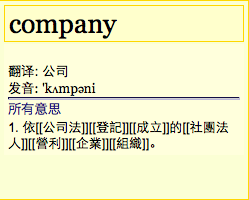
\includegraphics[scale=0.8]{./tooltip}
  \caption{DiCE Translator tooltip}
  \label{tooltip}
\end{figure}
\begin{figure}[htbp]
  \centering
  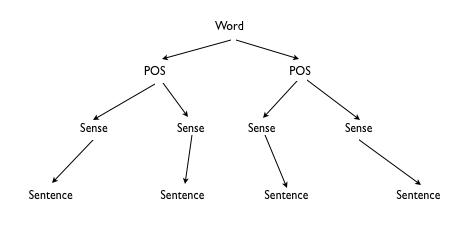
\includegraphics[scale=0.8]{./schema}
  \caption{Database Schema}
  \label{schema}
\end{figure}
\paragraph{}
From the extraction process, we extracted more than 47,000 English words and more than 3,000 Chinese words. Yet, it was all only about retrieving dictionary information, that from these information, we are unable to differentiate the senses so that they match the context in the sentence on a webpage. In other words, like the example mentioned earlier, we do not want \textit{interest} in ``interest rate'' to be interpreted as \begin{CJK}{UTF8}{gbsn}兴趣\end{CJK}.
\paragraph{}
What we want to do for DiCE is to make it ``smarter'' by being able to translate relevantly in terms of senses and context. For that, we intend to implement the following two methods of WSD.

\subsection{Supervised English All-words Word Sense Disambiguation}
\label{itmakessense}
\paragraph{}
\textit{It Makes Sense} (IMS) is a supervised English all-words WSD System introduced by Zhong \& Ng \cite{itmakessense}. It is a flexible system that allows users to customize it by integrating different preprocessing tools and additional features. There are generally 3 modules in IMS: Preprocessing, Feature \& Instance Extraction and Classification. The system accepts any input text. In the Preprocessing module, the OpenNLP toolkit is used by default. Sentences in the input are detected and split using a sentence splitter, and then tokenized into words, before POS tags are assigned to all tokens using OpenNLP's POS tagger. Then, the lemma form of each token is determined using a lemmatizer that is based on using the WordNet thesaurus. In the Extraction module, it makes use of 3 knowledge sources namely, POS Tags of Surrounding Words, Surrounding Words and Local Collocations. In general, the purpose of using these knowledges is to increase the accuracy of the the WSD. Finally in the Classification module, the IMS's classifier trains a model for each word type which has training data during the training process. The classifier as used by IMS is LIBLINEAR. In the testing process, the trained classification models will be applied to the test instances of the corresponding word types. If a test instance is not seen, IMS outputs the first sense found in the WordNet sense inventory.

\paragraph{}
We intend to utilize IMS as a back-end system for DiCE to disambiguate words selected by users on a webpage. The advantage of IMS is being able to handle longer text inputs, in sentences or paragraphs. However, we are limited to only English inputs, and might be required to use the database tables and Google Translate concurrently to translate to Chinese language.

\subsection{Word Sense Disambiguation using Wikipedia}
\paragraph{}
We make reference to Mihalcea's work \cite{wikipedia} on using Wikipedia for WSD. As mentioned in Section \ref{wikipedia}, we can utilize the annotations created by authors of Wikipedia to determine the sense of ambiguous words. Most importantly, for a word like \textit{interest}, a Wikipedia page would contain translations in various context. This will address the limitation highlighted in Section \ref{itmakessense}, that we can have more accurate English-to-Chinese translations that preserve context.
%\paragraph{}
%The real-time alternative approach would be to use the MediaWiki's APIs, for instance the Query API that allows retrieving all kinds of data from Wikipedia pages. The returned results would contain useful annotations and at the same time, access WordNet via its web interface to retrieve word sense information real-time.

%\section{Evaluation}
%\label{evaluation}
%\paragraph{}
%Lorem ipsum dolor sit amet, consectetur adipisicing elit, sed do eiusmod tempor incididunt ut labore et dolore magna aliqua. Ut enim ad minim veniam, quis nostrud exercitation ullamco laboris nisi ut aliquip ex ea commodo consequat. Duis aute irure dolor in reprehenderit in voluptate velit esse cillum dolore eu fugiat nulla pariatur. Excepteur sint occaecat cupidatat non proident, sunt in culpa qui officia deserunt mollit anim id est laborum.

\section{Conclusion}
\label{conclusion}
\paragraph{}
Word Sense Disambiguation is a very challenging task due the complexity of the human languages. There are various approaches, either by using formal dictionarys and lexical databases, or to induce the word senses by analyzing the words in a given text. One of the applications for WSD is making translations more accurate and relevant by retaining the original context, which is related to the goals of the DiCE Translator, a Firefox extension that allows users to translate text on a webpage from English to Chinese and vice versa. With DiCE, we hope to make language learning easier by providing translations for the language to be learnt. Other than providing definitions and sample sentence, we wish to make translations more meaningful and accurate by being able to retain the context of the text selected by users. For that we looked at a few WSD-related works. Notably, the approach introduced by Mihalcea \cite{wikipedia}, and the \textit{It Makes Sense} \cite{itmakessense} system have been considered to be integrated with the DiCE Translator. No formal evaluation has been performed and so what follows would be the implementation of these WSD systems, in order for us to move on into the Evaluation phase.
%\paragraph{}
%In this review we touched on the field of \textit{Word Sense Disambiguation} (\textit{WSD}). WSD is a very challenging task because it involves working with the complexity of human languages. First formulated as a distinct computational task during the 1940s, WSD is one of the oldest problems in computational linguistics. Weaver \cite{weaver} wrote in his memorandum, that if we examine text \textit{one} word at a time, it is impossible to determine the meaning of it. Only by looking at its surrounding words then can one decide its meaning.
%Among the four conventional approaches for WSD mentioned, \textit{Supervised} is undoubtly the most accurate in WSD. However, in order for Supervised to work reliably, it needs to work with a manually sense-tagged corpora, which is expensive to create or upgrade. Diab \& Resnik described a more practical method \cite{parallel} that uses a combination of an existing corpora, translations and word alignments to automate the creation of a sense-tagged corpora. Its advantage is it could be the automated solution to sense-tagging and annotation. For \textit{Unsupervised}, the approaches mentioned in Section \ref{wikipedia} and \ref{treematching} both share one thing in common: Web-based corpora. In both approaches, they adapted the Web-based corpora because it is dynamic and up-to-date. This mean their systems will be able to handle new words and new senses, which may help in overcoming the \textit{knowledge acquisition bottleneck}. However, there is one concern about retrieving senses information from such a large and open resource: Data inconsistency. But the authors of \cite{unsupervised} said that this problem would be negligible when using popular Web search engines to extract relevant Web pages.
%\paragraph{}
%Related to our topic of interest, it is notable that Lefever \& Hoste \cite{crosslingual} had demonstrated Cross Lingual WSD using parallel corpora from Europarl\footnote{http://www.statmt.org/europarl/}. However, the corpora used were mainly in European languages, not applicable when the languages we are focusing on are English and Chinese. There are many papers introducing methods to construct an English-Chinese parallel corpus (see \cite{Dalianis,sun,Baobao2004}, however not discussed in this review for the focus is on word senses). So maybe for our study in Cross Lingual WSD, we could look at these various methods of construct a parallel corpus, and also the method mentioned in Section \ref{parallel}.

%\paragraph{}
%In general, the characteristics mentioned in this review are \textit{accuracy}, \textit{flexible} (to handle new words \& senses) and \textit{unsupervised}. For that, we have studied some approaches and techniques that may give rise to these characteristics in WSD. Diab \& Resnik \cite{parallel} described a form of automated sense-tagging by analyzing an ambiguous word's translations in a second language. This introduces not only automation to sense-tagging, but also contributes to more \textit{accurate} translations between the languages in the parallel corpora. To be \textit{flexible}, the general idea is to adapt a Web-based resource for sense-extraction. Mihalcea described using Wikipedia for WSD \cite{wikipedia}. Advantages include it being publicly accurate in its contents, and it being exposed to new words and senses added by articles' authors regularly. While data inconsistency might be an issue here, it is flexible enough to handle ambiguous words that may not yet appear on formal dictionaries. As for \textit{unsupervised}, \cite{unsupervised} introduced an approach that determines the correct sense by on dependency knowledge. Although unsupervised, \cite{unsupervised} showed that its precision was pretty close to the supervised methods that were in their evaluation tests. As a whole, I believe that by integrating these techniques, a system would have accurate parallel corpora and word sense disambiguations, be adaptable to new words and senses in languages, and therefore, lead to improved bilingual translations.

%\paragraph{}
%Perhaps the next idea to consider is to go real-time for WSD. So far the above mentioned literatures did not touch on this idea, probably because of performance issues, for it can be easily inferred that the construction of large corpora could not possibly be achieved in a matter of seconds. While this poses yet another challenge not exclusive to the field of Word Sense Disambiguation, but as systems' performance are reaching new heights regularly, it should not be impossible in the near future.
%Relating back to our goal, these solutions could possibly integrate with the approach mentioned in Section \ref{parallel} to construct a dynamic sense-tagged corpus that could easily be updated, in order to handle new emerging words and senses in human languages.
%\\
%\\
%Finally, the techniques mentioned in Section \ref{wikipedia} and \ref{treematching} had proved to be quite accurate in disambiguating word senses. With precision rates of about 84\% \cite{wikipedia} and 73\% \cite{unsupervised} respectively, they performed outstandingly considering the fact that they are unsupervised approaches. Adapting to these techniques, combined with a fine created corpus, we could possibly make bilingual translations better and more accurate.

\bibliography{bibsource}
\end{document}













